% Created by tikzDevice version 0.10.1 on 2016-06-02 06:53:09
% !TEX encoding = UTF-8 Unicode
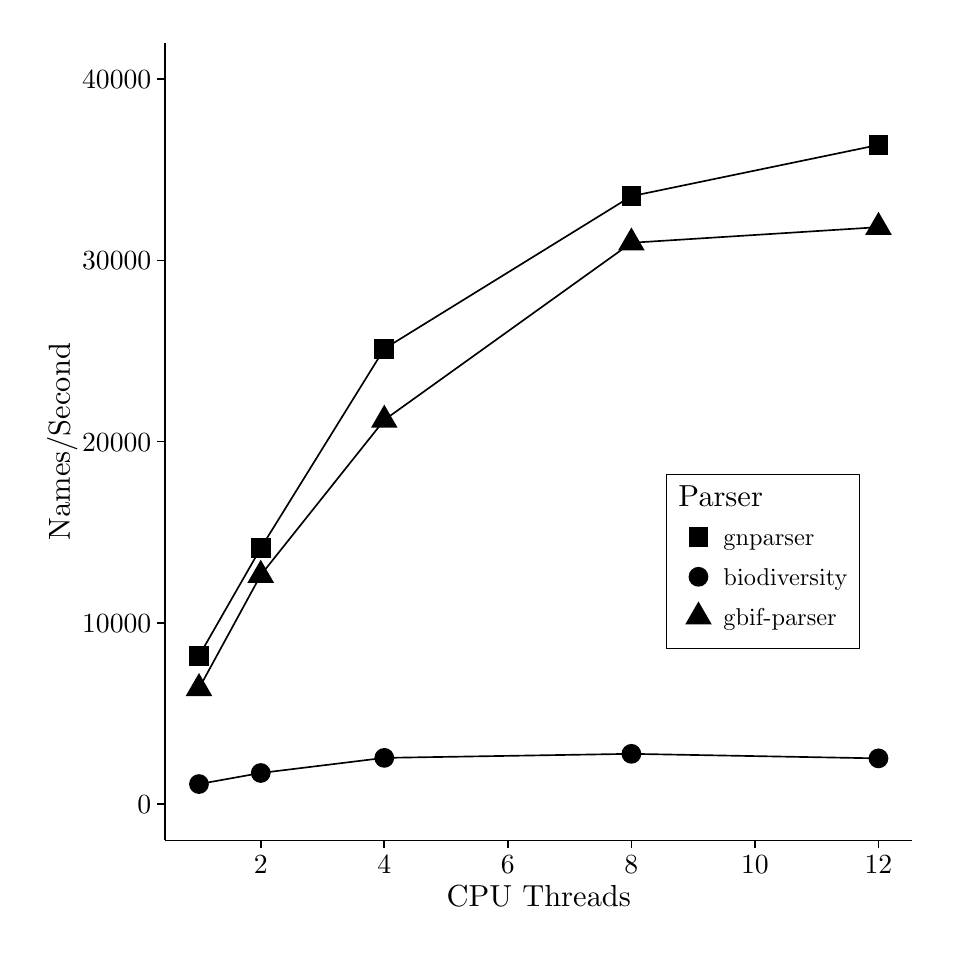
\begin{tikzpicture}[x=1pt,y=1pt]
\definecolor{fillColor}{RGB}{255,255,255}
\path[use as bounding box,fill=fillColor,fill opacity=0.00] (0,0) rectangle (325.21,325.21);
\begin{scope}
\path[clip] (  0.00,  0.00) rectangle (325.21,325.21);
\definecolor{drawColor}{RGB}{255,255,255}
\definecolor{fillColor}{RGB}{255,255,255}

\path[draw=drawColor,line width= 0.6pt,line join=round,line cap=round,fill=fillColor] (  0.00,  0.00) rectangle (325.21,325.21);
\end{scope}
\begin{scope}
\path[clip] ( 49.62, 31.51) rectangle (319.71,319.71);
\definecolor{fillColor}{RGB}{255,255,255}

\path[fill=fillColor] ( 49.62, 31.51) rectangle (319.71,319.71);
\definecolor{drawColor}{RGB}{255,255,255}

\path[draw=drawColor,line width= 0.3pt,line join=round] ( 49.62, 77.36) --
	(319.71, 77.36);

\path[draw=drawColor,line width= 0.3pt,line join=round] ( 49.62,142.86) --
	(319.71,142.86);

\path[draw=drawColor,line width= 0.3pt,line join=round] ( 49.62,208.36) --
	(319.71,208.36);

\path[draw=drawColor,line width= 0.3pt,line join=round] ( 49.62,273.86) --
	(319.71,273.86);

\path[draw=drawColor,line width= 0.3pt,line join=round] ( 61.90, 31.51) --
	( 61.90,319.71);

\path[draw=drawColor,line width= 0.3pt,line join=round] (106.54, 31.51) --
	(106.54,319.71);

\path[draw=drawColor,line width= 0.3pt,line join=round] (151.18, 31.51) --
	(151.18,319.71);

\path[draw=drawColor,line width= 0.3pt,line join=round] (195.83, 31.51) --
	(195.83,319.71);

\path[draw=drawColor,line width= 0.3pt,line join=round] (240.47, 31.51) --
	(240.47,319.71);

\path[draw=drawColor,line width= 0.3pt,line join=round] (285.12, 31.51) --
	(285.12,319.71);

\path[draw=drawColor,line width= 0.6pt,line join=round] ( 49.62, 44.61) --
	(319.71, 44.61);

\path[draw=drawColor,line width= 0.6pt,line join=round] ( 49.62,110.11) --
	(319.71,110.11);

\path[draw=drawColor,line width= 0.6pt,line join=round] ( 49.62,175.61) --
	(319.71,175.61);

\path[draw=drawColor,line width= 0.6pt,line join=round] ( 49.62,241.11) --
	(319.71,241.11);

\path[draw=drawColor,line width= 0.6pt,line join=round] ( 49.62,306.61) --
	(319.71,306.61);

\path[draw=drawColor,line width= 0.6pt,line join=round] ( 84.22, 31.51) --
	( 84.22,319.71);

\path[draw=drawColor,line width= 0.6pt,line join=round] (128.86, 31.51) --
	(128.86,319.71);

\path[draw=drawColor,line width= 0.6pt,line join=round] (173.51, 31.51) --
	(173.51,319.71);

\path[draw=drawColor,line width= 0.6pt,line join=round] (218.15, 31.51) --
	(218.15,319.71);

\path[draw=drawColor,line width= 0.6pt,line join=round] (262.79, 31.51) --
	(262.79,319.71);

\path[draw=drawColor,line width= 0.6pt,line join=round] (307.44, 31.51) --
	(307.44,319.71);
\definecolor{drawColor}{RGB}{0,0,0}

\path[draw=drawColor,line width= 0.6pt,line join=round] ( 61.90, 51.89) --
	( 84.22, 55.89) --
	(128.86, 61.35) --
	(218.15, 62.81) --
	(307.44, 61.17);

\path[draw=drawColor,line width= 0.6pt,line join=round] ( 61.90, 86.46) --
	( 84.22,127.40) --
	(128.86,183.44) --
	(218.15,247.48) --
	(307.44,253.12);

\path[draw=drawColor,line width= 0.6pt,line join=round] ( 61.90, 98.18) --
	( 84.22,137.13) --
	(128.86,209.18) --
	(218.15,264.31) --
	(307.44,282.83);
\definecolor{fillColor}{RGB}{0,0,0}

\path[fill=fillColor] ( 58.33, 94.61) --
	( 65.47, 94.61) --
	( 65.47,101.75) --
	( 58.33,101.75) --
	cycle;

\path[fill=fillColor] ( 80.65,133.56) --
	( 87.79,133.56) --
	( 87.79,140.70) --
	( 80.65,140.70) --
	cycle;

\path[fill=fillColor] (125.29,205.61) --
	(132.43,205.61) --
	(132.43,212.75) --
	(125.29,212.75) --
	cycle;

\path[fill=fillColor] (214.58,260.74) --
	(221.72,260.74) --
	(221.72,267.88) --
	(214.58,267.88) --
	cycle;

\path[fill=fillColor] (303.87,279.27) --
	(311.01,279.27) --
	(311.01,286.40) --
	(303.87,286.40) --
	cycle;

\path[fill=fillColor] ( 61.90, 92.01) --
	( 66.70, 83.69) --
	( 57.09, 83.69) --
	cycle;

\path[fill=fillColor] ( 84.22,132.95) --
	( 89.02,124.62) --
	( 79.41,124.62) --
	cycle;

\path[fill=fillColor] (128.86,188.99) --
	(133.67,180.66) --
	(124.06,180.66) --
	cycle;

\path[fill=fillColor] (218.15,253.03) --
	(222.96,244.71) --
	(213.34,244.71) --
	cycle;

\path[fill=fillColor] (307.44,258.67) --
	(312.24,250.35) --
	(302.63,250.35) --
	cycle;

\path[fill=fillColor] ( 61.90, 51.89) circle (  3.57);

\path[fill=fillColor] ( 84.22, 55.89) circle (  3.57);

\path[fill=fillColor] (128.86, 61.35) circle (  3.57);

\path[fill=fillColor] (218.15, 62.81) circle (  3.57);

\path[fill=fillColor] (307.44, 61.17) circle (  3.57);
\end{scope}
\begin{scope}
\path[clip] (  0.00,  0.00) rectangle (325.21,325.21);
\definecolor{drawColor}{RGB}{0,0,0}

\path[draw=drawColor,line width= 0.6pt,line join=round] ( 49.62, 31.51) --
	( 49.62,319.71);
\end{scope}
\begin{scope}
\path[clip] (  0.00,  0.00) rectangle (325.21,325.21);
\definecolor{drawColor}{RGB}{0,0,0}

\node[text=drawColor,anchor=base east,inner sep=0pt, outer sep=0pt, scale=  1.00] at ( 44.67, 41.17) {0};

\node[text=drawColor,anchor=base east,inner sep=0pt, outer sep=0pt, scale=  1.00] at ( 44.67,106.67) {10000};

\node[text=drawColor,anchor=base east,inner sep=0pt, outer sep=0pt, scale=  1.00] at ( 44.67,172.17) {20000};

\node[text=drawColor,anchor=base east,inner sep=0pt, outer sep=0pt, scale=  1.00] at ( 44.67,237.67) {30000};

\node[text=drawColor,anchor=base east,inner sep=0pt, outer sep=0pt, scale=  1.00] at ( 44.67,303.17) {40000};
\end{scope}
\begin{scope}
\path[clip] (  0.00,  0.00) rectangle (325.21,325.21);
\definecolor{drawColor}{RGB}{0,0,0}

\path[draw=drawColor,line width= 0.6pt,line join=round] ( 46.87, 44.61) --
	( 49.62, 44.61);

\path[draw=drawColor,line width= 0.6pt,line join=round] ( 46.87,110.11) --
	( 49.62,110.11);

\path[draw=drawColor,line width= 0.6pt,line join=round] ( 46.87,175.61) --
	( 49.62,175.61);

\path[draw=drawColor,line width= 0.6pt,line join=round] ( 46.87,241.11) --
	( 49.62,241.11);

\path[draw=drawColor,line width= 0.6pt,line join=round] ( 46.87,306.61) --
	( 49.62,306.61);
\end{scope}
\begin{scope}
\path[clip] (  0.00,  0.00) rectangle (325.21,325.21);
\definecolor{drawColor}{RGB}{0,0,0}

\path[draw=drawColor,line width= 0.6pt,line join=round] ( 49.62, 31.51) --
	(319.71, 31.51);
\end{scope}
\begin{scope}
\path[clip] (  0.00,  0.00) rectangle (325.21,325.21);
\definecolor{drawColor}{RGB}{0,0,0}

\path[draw=drawColor,line width= 0.6pt,line join=round] ( 84.22, 28.76) --
	( 84.22, 31.51);

\path[draw=drawColor,line width= 0.6pt,line join=round] (128.86, 28.76) --
	(128.86, 31.51);

\path[draw=drawColor,line width= 0.6pt,line join=round] (173.51, 28.76) --
	(173.51, 31.51);

\path[draw=drawColor,line width= 0.6pt,line join=round] (218.15, 28.76) --
	(218.15, 31.51);

\path[draw=drawColor,line width= 0.6pt,line join=round] (262.79, 28.76) --
	(262.79, 31.51);

\path[draw=drawColor,line width= 0.6pt,line join=round] (307.44, 28.76) --
	(307.44, 31.51);
\end{scope}
\begin{scope}
\path[clip] (  0.00,  0.00) rectangle (325.21,325.21);
\definecolor{drawColor}{RGB}{0,0,0}

\node[text=drawColor,anchor=base,inner sep=0pt, outer sep=0pt, scale=  1.00] at ( 84.22, 19.68) {2};

\node[text=drawColor,anchor=base,inner sep=0pt, outer sep=0pt, scale=  1.00] at (128.86, 19.68) {4};

\node[text=drawColor,anchor=base,inner sep=0pt, outer sep=0pt, scale=  1.00] at (173.51, 19.68) {6};

\node[text=drawColor,anchor=base,inner sep=0pt, outer sep=0pt, scale=  1.00] at (218.15, 19.68) {8};

\node[text=drawColor,anchor=base,inner sep=0pt, outer sep=0pt, scale=  1.00] at (262.79, 19.68) {10};

\node[text=drawColor,anchor=base,inner sep=0pt, outer sep=0pt, scale=  1.00] at (307.44, 19.68) {12};
\end{scope}
\begin{scope}
\path[clip] (  0.00,  0.00) rectangle (325.21,325.21);
\definecolor{drawColor}{RGB}{0,0,0}

\node[text=drawColor,anchor=base,inner sep=0pt, outer sep=0pt, scale=  1.10] at (184.67,  7.70) {CPU Threads};
\end{scope}
\begin{scope}
\path[clip] (  0.00,  0.00) rectangle (325.21,325.21);
\definecolor{drawColor}{RGB}{0,0,0}

\node[text=drawColor,rotate= 90.00,anchor=base,inner sep=0pt, outer sep=0pt, scale=  1.10] at ( 15.28,175.61) {Names/Second};
\end{scope}
\begin{scope}
\path[clip] (  0.00,  0.00) rectangle (325.21,325.21);
\definecolor{drawColor}{RGB}{0,0,0}
\definecolor{fillColor}{RGB}{255,255,255}

\path[draw=drawColor,line width= 0.3pt,line join=round,line cap=round,fill=fillColor] (230.90,100.84) rectangle (300.49,163.93);
\end{scope}
\begin{scope}
\path[clip] (  0.00,  0.00) rectangle (325.21,325.21);
\definecolor{drawColor}{RGB}{0,0,0}

\node[text=drawColor,anchor=base west,inner sep=0pt, outer sep=0pt, scale=  1.10] at (235.17,152.08) {Parser};
\end{scope}
\begin{scope}
\path[clip] (  0.00,  0.00) rectangle (325.21,325.21);
\definecolor{drawColor}{RGB}{255,255,255}
\definecolor{fillColor}{RGB}{255,255,255}

\path[draw=drawColor,line width= 0.6pt,line join=round,line cap=round,fill=fillColor] (235.17,134.02) rectangle (249.62,148.47);
\end{scope}
\begin{scope}
\path[clip] (  0.00,  0.00) rectangle (325.21,325.21);
\definecolor{fillColor}{RGB}{0,0,0}

\path[fill=fillColor] (238.83,137.67) --
	(245.96,137.67) --
	(245.96,144.81) --
	(238.83,144.81) --
	cycle;
\end{scope}
\begin{scope}
\path[clip] (  0.00,  0.00) rectangle (325.21,325.21);
\definecolor{drawColor}{RGB}{255,255,255}
\definecolor{fillColor}{RGB}{255,255,255}

\path[draw=drawColor,line width= 0.6pt,line join=round,line cap=round,fill=fillColor] (235.17,119.56) rectangle (249.62,134.02);
\end{scope}
\begin{scope}
\path[clip] (  0.00,  0.00) rectangle (325.21,325.21);
\definecolor{fillColor}{RGB}{0,0,0}

\path[fill=fillColor] (242.39,126.79) circle (  3.57);
\end{scope}
\begin{scope}
\path[clip] (  0.00,  0.00) rectangle (325.21,325.21);
\definecolor{drawColor}{RGB}{255,255,255}
\definecolor{fillColor}{RGB}{255,255,255}

\path[draw=drawColor,line width= 0.6pt,line join=round,line cap=round,fill=fillColor] (235.17,105.11) rectangle (249.62,119.56);
\end{scope}
\begin{scope}
\path[clip] (  0.00,  0.00) rectangle (325.21,325.21);
\definecolor{fillColor}{RGB}{0,0,0}

\path[fill=fillColor] (242.39,117.88) --
	(247.20,109.56) --
	(237.59,109.56) --
	cycle;
\end{scope}
\begin{scope}
\path[clip] (  0.00,  0.00) rectangle (325.21,325.21);
\definecolor{drawColor}{RGB}{0,0,0}

\node[text=drawColor,anchor=base west,inner sep=0pt, outer sep=0pt, scale=  0.88] at (251.43,138.21) {gnparser};
\end{scope}
\begin{scope}
\path[clip] (  0.00,  0.00) rectangle (325.21,325.21);
\definecolor{drawColor}{RGB}{0,0,0}

\node[text=drawColor,anchor=base west,inner sep=0pt, outer sep=0pt, scale=  0.88] at (251.43,123.76) {biodiversity};
\end{scope}
\begin{scope}
\path[clip] (  0.00,  0.00) rectangle (325.21,325.21);
\definecolor{drawColor}{RGB}{0,0,0}

\node[text=drawColor,anchor=base west,inner sep=0pt, outer sep=0pt, scale=  0.88] at (251.43,109.30) {gbif-parser};
\end{scope}
\end{tikzpicture}
